\documentclass[12pt]{article}

\usepackage{algorithm}
\usepackage[noend]{algorithmic}
\usepackage[italian]{babel}
\usepackage{caption}
\usepackage{enumitem}
\usepackage{float}
\usepackage{fullpage}
\usepackage{graphicx}
\usepackage[colorlinks=true, urlcolor=blue]{hyperref}
\usepackage[utf8]{inputenc}
\usepackage{minted}
\usepackage{subcaption}

% Hacks needed to get the algorithm package to work.
\floatname{algorithm}{Algoritmo}
\renewcommand{\algorithmicrequire}{\textbf{Input:}}

\title{Progetto del corso Sistemi Distribuiti: Paradigmi e Modelli, 2012/2013}
\author{
	Jacopo Notarstefano\\
	\texttt{jacopo [dot] notarstefano [at] gmail.com}
}
\date{}

% http://tex.stackexchange.com/a/4304/10806
\newcommand{\cpp}{C\nolinebreak\hspace{-.05em}\raisebox{.4ex}{\tiny\bf +}\nolinebreak\hspace{-.10em}\raisebox{.4ex}{\tiny\bf +}}
\newcommand{\mpp}{Magick\nolinebreak\hspace{-.05em}\raisebox{.4ex}{\tiny\bf +}\nolinebreak\hspace{-.10em}\raisebox{.4ex}{\tiny\bf +}}

\begin{document}
  \maketitle
    \section{Introduzione}

    Scopo di questo progetto è dare un'implementazione sequenziale e una
    parallela di una soluzione al problema dell'Histogram Thresholding, per
    poi confrontarne le performance sia fra esse sia con i modelli teorici.

    Entrambe le implementazioni sono realizzate in \cpp; in particolare
    quella parallela è data in termini di parallel skeleton, più nello
    specifico quelli forniti dal framework 
    \href{http://sketo.ipl-lab.org/}{\underline{SkeTo}}.

    SkeTo è uno skeleton framework in cui dichiarazione e istanziazione degli
    skeleton avvengono allo stesso tempo. I metodi offerti dalle classi
    astratte del framework, implementate in termini di template, sono quelli
    tipici della programmazione funzionale, come \texttt{map}, \texttt{reduce}
    e \texttt{scan}. Queste caratteristiche rendono molto compatto il codice:
    in effetti l'intero codice non funzionale parallelo di
    \texttt{src/parallel.cpp} ammonta a \(63\) righe commenti inclusi, di cui
    appena \(3\) chiamate di libreria.

    Il codice non funzionale sequenziale di \texttt{src/sequential.cpp} \`e
    un ordinario programma \cpp. La struttura delle due implementazioni \`e
    molto simile: questo perch\'e il business code dell'applicazione \`e
    stato incapsulato nella classe \texttt{Job}, la cui interfaccia \`e
    definita in \texttt{src/job.h} e la cui implementazione in
    \texttt{src/job.cpp}.

    Per prima cosa presentiamo il problema dell'Histogram Thresholding e
    descriviamo l'algoritmo risolutivo implementato. In seguito descriviamo in
    maggiore dettaglio le scelte implementative adottate durante lo sviluppo.
    Parte centrale del lavoro \`e il confronto delle performance con le
    previsioni teoriche, seguito da una dimostrazione dei risultati ottenuti
    dal programma. Concludiamo con un manuale d'uso che contiene le rule
    definite nel \texttt{Makefile} e altri script disponibili.

    \section{Il problema dell'Histogram Thresholding}

    Siano \texttt{I} un'immagine e \texttt{p} una percentuale. Supponiamo di 
    avere accesso ai singoli pixel dell'immagine, e denotiamo con 
    \texttt{I[i][j]} il pixel alla riga \texttt{i} e colonna \texttt{j}.
    Il problema dell'Histogram Thresholding consiste nel restituire
    un'immagine in bianco e nero \texttt{BW} tale che il pixel
    \texttt{BW[i][j]} sia bianco se il pixel \texttt{I[i][j]} è più luminoso
    di \texttt{p}\% pixel dell'immagine originaria, nero altrimenti.\footnote{
    Osserviamo che in letteratura esistono più definizioni di luminosità di 
    un pixel; le soluzioni proposte usano la coordinata \texttt{L} nello 
    spazio colori \texttt{HSL}.}

    L'algoritmo di risoluzione implementato visita ogni pixel, ne calcola la
    luminosit\`a e la scrive in un vettore. Successivamente lo ordina e
    ricava la luminosit\`a soglia per la percentuale \texttt{p}. Infine visita
    nuovamente ogni pixel dell'immagine originaria e, confrontando con il
    valore soglia precedentemente ottenuto, assegna al corrispondente pixel
    dell'immagine risultante il colore bianco o nero. Pi\`u precisamente
    abbiamo il seguente:

    \begin{algorithm}
        \caption{\textsc{Na\"ive Histogram Thresholding}}
        \begin{algorithmic}[1]
            \REQUIRE \texttt{luminosities} \(=\) \texttt{[]}, \texttt{I} immagine di larghezza \texttt{imageWidth} e altezza \texttt{imageHeight}
            \FOR{\texttt{i} \(\le\) \texttt{imageWidth}}
                \FOR{\texttt{j} \(\le\) \texttt{imageHeight}}
                    \STATE \texttt{luminosities.push(I[i][j].luminosity())}
                \ENDFOR
            \ENDFOR
            \STATE \texttt{luminosities.sort()}
            \STATE \texttt{threshold} \(\leftarrow\) \texttt{luminosities[luminosities.length() * p / 100]}
            \FOR{\texttt{i} \(\le\) \texttt{imageWidth}}
                \FOR{\texttt{j} \(\le\) \texttt{imageHeight}}
                    \IF{\texttt{I[i][j].luminosity()} \(>\) \texttt{threshold}}
                        \STATE \texttt{BW[i][j]} \(\leftarrow\) \texttt{white}
                    \ELSE
                        \STATE \texttt{BW[i][j]} \(\leftarrow\) \texttt{black}
                    \ENDIF
                \ENDFOR
            \ENDFOR
            \RETURN \texttt{BW}
        \end{algorithmic}
    \end{algorithm}

    \section{Descrizione delle implementazioni}

    Abbiamo posto particolare enfasi nella divisione fra codice funzionale e
    non funzionale; in particolare il business code dell'applicazione è
    interamente astratto nella classe \texttt{Job}, di cui diamo di seguito
    l'interfaccia:

    \inputminted[]{c++}{src/job.h}

    Osserviamo che i metodi \texttt{execute} e \texttt{writeResult} hanno
    come tipo di ritorno \texttt{Job}; in effetti questi metodi ritornano
    l'oggetto stesso. Ciò consente di usarli in \texttt{sequential.cpp} come
    se avessero tipo di ritorno \texttt{void} (cio\`e ignorandone il valore
    di ritorno), e in \texttt{parallel.cpp}, come argomento di
    \texttt{generate} e \texttt{map}, dopo averli astratti in opportuni
    function object come nel seguente esempio:

    \inputminted[]{c++}{tex/src/function-object.cpp}

    Come gi\`a ricordato l'implementazione parallela si avvale di SkeTo, in
    particolare la versione \texttt{1.1}. Esiste una versione pi\`u aggiornata,
    la \texttt{1.50pre}, scartata perch\'e ad oggi priva di documentazione.
    Internamente SkeTo si avvale di un'implementazione disponibile di MPI;
    quella utilizzata da questo progetto \`e la distribuzione
    \href{http://www.mpich.org}{\underline{MPICH}} versione \texttt{3.0.4}. 
    Infine la lettura e scrittura delle immagini sono interamente delegate alla
    libreria \href{http://www.imagemagick.org/script/index.php}{\underline{ImageMagick}}
    tramite \href{http://www.imagemagick.org/script/magick++.php}{\underline{\mpp}},
    la sua API per \cpp, versione \texttt{6.8.6-1}.

    \section{Valutazione delle performance}

    \section{Valutazione dei risultati}

    L'algoritmo implementato nel file \texttt{src/job.cpp} produce i
    seguenti risultati al variare della soglia \texttt{p}:

    \begin{figure}[H]
      \centering
      \begin{subfigure}[b]{0.33\textwidth}
        \centering
        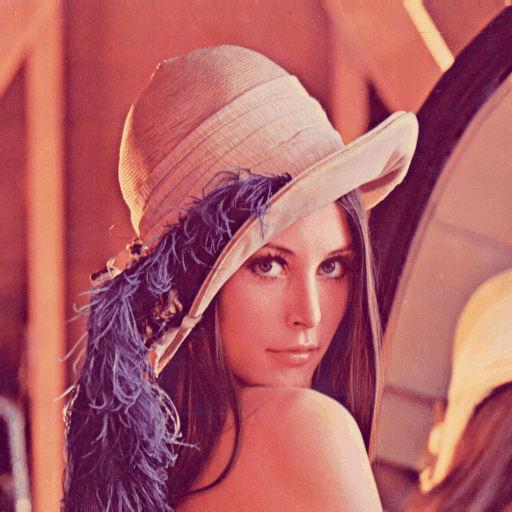
\includegraphics[width=\textwidth]{tex/img/lena.png}
        \caption*{Originale}
      \end{subfigure}
      \hspace{0.15\textwidth}
      \begin{subfigure}[b]{0.33\textwidth}
        \centering
        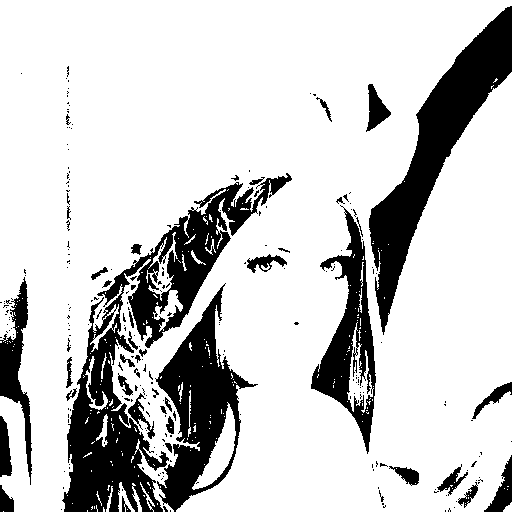
\includegraphics[width=\textwidth]{img/lena-threshold-20.png}
        \caption*{\texttt{p }\( = 20\%\)}
      \end{subfigure}

      \vspace{0.02\textwidth}

      \begin{subfigure}[b]{0.33\textwidth}
        \centering
        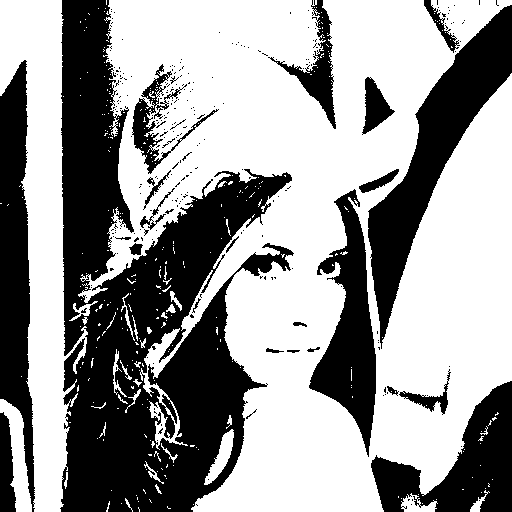
\includegraphics[width=\textwidth]{img/lena-threshold-40.png}
        \caption*{\texttt{p }\( = 40\%\)}
      \end{subfigure}
      \hspace{0.15\textwidth}
      \begin{subfigure}[b]{0.33\textwidth}
        \centering
        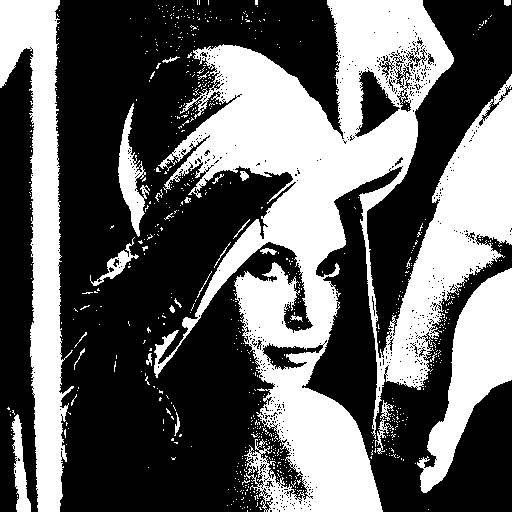
\includegraphics[width=\textwidth]{img/lena-threshold-60.png}
        \caption*{\texttt{p }\( = 60\%\)}
      \end{subfigure}

      \vspace{0.02\textwidth}

      \begin{subfigure}[b]{0.33\textwidth}
        \centering
        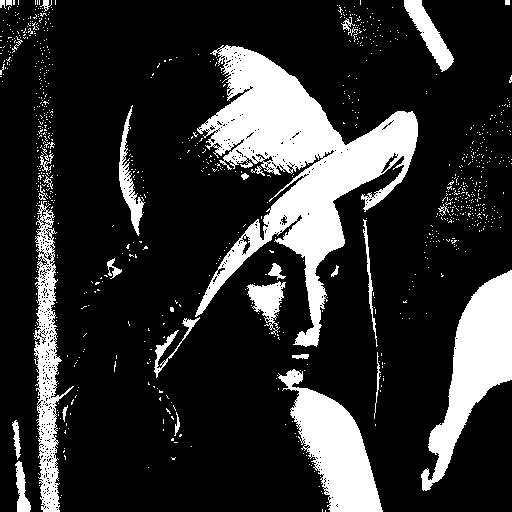
\includegraphics[width=\textwidth]{img/lena-threshold-80.png}
        \caption*{\texttt{p }\( = 80\%\)}
      \end{subfigure}
      \hspace{0.15\textwidth}
      \begin{subfigure}[b]{0.33\textwidth}
        \centering
        
\includegraphics[width=\textwidth]{img/lena-threshold-99.png}
        \caption*{\texttt{p }\( = 99\%\)}
      \end{subfigure}
    \end{figure}

    È inoltre possibile creare, usando l'utility \texttt{convert} di
    ImageMagick, una gif animata i cui frame siano le immagini risultanti
    al variare della soglia da \(0\) a \(99\). Per ottenerla \`e sufficiente
    invocare la rule \texttt{make gif} del \texttt{Makefile} oppure visitare il
    seguente indirizzo: \href{http://raw.github.com/jacquerie/SPM/master/lena.gif}{\underline{http://raw.github.com/jacquerie/SPM/master/lena.gif}}.

  \appendix
    \section{Manuale d'uso}
      \subsection{Makefile}

      \begin{description}
        \item[\texttt{all}:] Invoca le rule \texttt{gif}, \texttt{parallel}, \texttt{sequential} e \texttt{tex}
        \item[\texttt{clean}:] Rimuove i file generati dalle rule \texttt{gif}, \texttt{parallel}, \texttt{sequential} e \texttt{tex}.
        \item[\texttt{gif}:] Genera una gif animata i cui frame sono le
          immagini risultanti al variare della soglia \texttt{p} da \(0\) a
          \(99\). Richiede l'installazione di ImageMagick e che \texttt{convert}
          sia nel \texttt{PATH}.
        \item[\texttt{parallel}:] Compila con \texttt{sketocxx}
          l'implementazione parallela. Richiede l'installazione di SkeTo, una
          distribuzione di MPI compatibile e ImageMagick.
        \item[\texttt{sequential}:] Compila con \texttt{g++} l'implementazione
          sequenziale. Richiede l'installazione di ImageMagick.
        \item[\texttt{tex}:] Compila con \texttt{pdflatex} il presente
          documento. Richiede l'installazione di \texttt{pdflatex} e del
          pacchetto Python \href{http://pygments.org}{\underline{pygments}}.
      \end{description}

      \subsection{Eseguibili}

      \begin{description}
        \item[\texttt{./sequential numberOfJobs}:] Esegue \texttt{sequential}
          su \texttt{numberOfJobs} istanze del problema dell'Histogram
          Thresholding. Stampa su \texttt{stdout} una coppia separata da uno
          spazio in cui il primo numero \`e \texttt{numberOfJobs} e il secondo
          il tempo in secondi impiegato da \texttt{sequential} a meno di
          operazioni di lettura e scrittura sul file system. 
        \item[\texttt{./test\_parallel [numberOfJobs=10]}:] Aggiunge in coda al file
          \texttt{parallel.dat} i risultati di \(10\) invocazioni su \texttt{NP}
          processi, per \texttt{NP} che varia da \(1\) a \(16\),
          dell'implementazione parallela su istanze di taglia
          \texttt{numberOfJobs}. I risultati sono riportati come triple separate
          da spazi in cui il primo numero \`e \texttt{NP}, il secondo
          \texttt{numberOfJobs} e il terzo il tempo impiegato a meno di
          letture e scritture sul file system.
        \item[\texttt{./test\_sequential [numberOfJobs=10]}:] Invoca \(10\)
          volte \texttt{./sequential numberOfJobs} con valore di default \(10\),
          redirigendo \texttt{stdout} sul file \texttt{sequential.dat}.
      \end{description}

      Esiste infine la possibilit\`a di invocare direttamente
      \texttt{./parallel} con la sintassi
      \texttt{sketorun -np NP ./parallel numberOfJobs}, in cui \texttt{NP} \`e
      il numero di processi che si desiderano far partire.

      \subsection{Licenza}

      Il codice \`e rilasciato con \href{http://opensource.org/licenses/MIT}{\underline{licenza MIT}}
      ed \`e disponibile su \href{https://github.com/jacquerie/SPM}{\underline{Github}}.
\end{document}

